\chapter{Matériels et Méthodes}

\section{Flux de travail}

Pour réaliser le jeu de données nécessaire à l'entrainement de notre réseau de neurone,
nous avons utilisé le site Xeno-Canto \cite{XenoCanto}. Celui-ci recense un grand nombre de chants d'oiseau
de différentes espèces enregistrés par des utilisateurs.
Cependant, les chants d'oiseaux enregistrés possèdent des caractéristiques différentes (durée d'enregistrement,
format d'enregistrement, fréquence d'échantilonnage, bruit de fond).
Notre premier défi a donc été de créer un jeu de données permettant 
d'obtenir des résultats corrects. 
Pour cela, nous nous sommes fixé pour objectif d'obtenir une précision supérieure à 80\% sur les données de test
avec un réseau de neurone de type M5 \cite{M5}.
Cela nous permet entre autre de valider notre jeu de données. 
Nous avons donc suivi une approche itérative Figure \ref{graph:iterative_workflow}

\begin{figure}[!ht]
  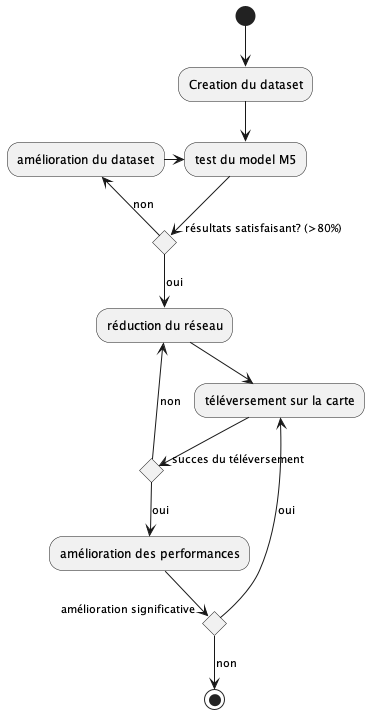
\includegraphics[width=0.5\textwidth]{iterative_workflow}
  \centering
  \caption{Workflow Iteratif}
  \label{graph:iterative_workflow}
\end{figure}

À chaque itération, nous avons essayé d'obtenir une meilleure précision qu'à l'itération précédente.
Notre première approche a consisté à récupérer le son de 10 espèces d'oiseaux depuis Xeno-Canto puis
à les convertir en .wav avant de tester le réseau de neurone M5 dessus.

Pour ce faire nous avons développé un script de récupération de données (scrapping) en Python nous permettant de sélectionner les espèces 
que nous voulions télécharger depuis le site. Lors de la récupération des sons, nous avons choisi de laisser 
un délai de 1 seconde entre chaque téléchargement pour ne pas surcharger le site. Nous avons également utilisé un script 
de conversion des fichiers en wav et de resampling en 16 000 Hz. Les scripts utilisés sont disponibles sur
notre \href{https://github.com/SamiElkateb/embedded_ai_project}{repository GitHub} \cite{Repository}.

Cette approche ne nous a malheureusement pas permis d'obtenir des résultats satisfaisants. En effet, 
le réseau de neurone M5 ne nous permettait d'obtenir qu'une précision de 20\%.

Nous avons donc choisis de découper les sons de notre jeu de données en échantillons de 1 seconde.
Ce traitement nous a permis d'obtenir une amélioration de 20\% de la précision 
du réseau de neurone M5 qui est passée de 20\% à 40\%. 

Cependant, nous pouvons trouver plusieurs défauts à cette approche. La principale est que sur les enregistrements de plusieurs minutes,
les chants d'oiseau ne sont pas constant et il existe des périodes de silence. 
Nous en déduisons qu'une des raisons de la mauvaise performance de notre réseau de neurone 
et que certains échantillons ne contiennent pas de chants d'oiseaux. 

\pagebreak
Nous avons réfléchi à plusieurs façons de résoudre ce problème : 
\begin{itemize}
  \item Contrôler manuellement la présence ou non de chant d'oiseau 
  \item Filtrer les sons automatiquement et supprimer les silences
  \item Entrainer un algorithme non supervisé pour permettre de détecter les échantillons potentiellement mal labélisés
\end{itemize}

Pour des raisons de temps et d'efficacité, nous avons choisi la seconde approche. Pour cela, nous avons
utilisé le script "Silence Remove" proposé dans l'article \emph{Audio Processing and Remove Silence using Python} \cite{DataCleaning}

 
Cette approche nous a finalement permis d'obtenir un taux de précision adéquat de 82\% sur les données de tests.
Nous avons donc choisi d'utilisé cette solution pour la création de notre jeu de données.

Par la suite, il a été nécessaire de réduire la taille du réseau de neurone ainsi que la quantité de données le traversant.
Nous avons donc réduit le réseau de neurone M5 de manière itérative, en essayant de garder une précision aussi élevée que possible.
Ceci a permis de téléverser sur la carte STM32 pour tester notre modèle.
Ce qui finalise notre flux  de travail Figure \ref{graph:final_workflow}.

\begin{figure}[!ht]
  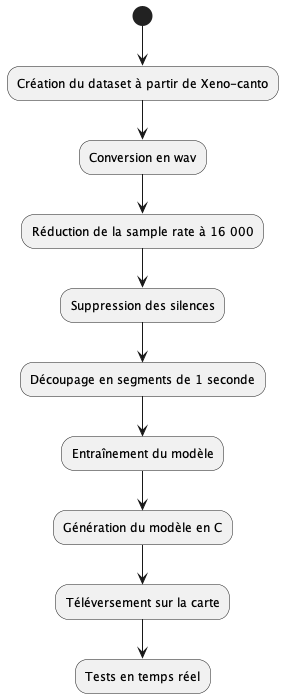
\includegraphics[width=0.4\textwidth]{final_workflow}
  \centering
  \caption{Workflow Final}
  \label{graph:final_workflow}
\end{figure}


\section{Jeu de données}
Notre jeu de données final contient un total de 33 105 échantillons de 1 seconde 
répartis de manière équitable sur 10 classes. 
Celui-ci est disponible sur notre \href{https://drive.google.com/file/d/1zVLOBS-vfTlgu_EdVVaLhvU9dm-XX1qR/view?usp=sharing}{Google Drive}\cite{Dataset}

\begin{center}
  \begin{tabular}{ |c|c|c|c| }
   \hline
   \multicolumn{4}{|c|}{Jeu de données : Espèces d'oiseaux} \\
   \hline
    Nom Français & Nom Anglais & Espèce & Nombre d'échantillons\\
   \hline
    Alouette des champs & Eurasian skylark & Alauda arvensis & 3 381\\
    Bruant jaune & Yellowhammer & Emberiza citrinella & 3 278\\
    Bruant zizi & Cirl bunting & Emberiza cirlus & 3 305\\
    Coucou gris & Common cuckoo & Cuculus canorus & 3 323\\
    Effraie des clochers & Barn owl & Tyto alba & 3 254\\
    Faucon crécerelle & Common kestrel & Falco tinnunculus & 3 311\\
    Fauvette des jardins & Garden warbler & Sylvia borin & 3 398\\
    Gobemouche gris & Spotted flycatcher & Muscicapa striata & 3 319\\
    Grèbe castagneux & Little grebe & Tachybaptus ruficollis & 3 167\\
    Hirondelle de fenêtre & Common house martin & Delichon urbicum & 3 369\\
   \hline
  \end{tabular}
\end{center}

\section{Description du CNN}

Pour pouvoir déployer le CNN sur la carte STM32 NUCLEO-L476RG, il a été nécessaire 
de minimiser les ressources utilisées par notre réseau de neurone. Pour cela les paramètres à prendre en compte sont
la taille et la quantité de données utilisée par le réseau (RAM et ROM) ainsi que le nombre 
de paramètres du réseau (temps de calcul).

Pour réduire la taille et le nombre de paramètres de notre réseau, nous avons diminué le nombre de filtres de nos
Conv1D. Nous avons ensuite utilisé un MaxPool en entrée du réseau pour réduire la quantité de données initiales. 
Ceci a permi de ne pas dépasser la RAM disponible sur la carte et de réduire le nombre de paramètres à 12 234.

\begin{center}
  \begin{tabular}{ |c|}
   \hline
    Input: 16000x1\\
   \hline
    Maxpool: 10x1 (output: 1600 × n)\\
   \hline
    conv1d [80/4, 32]\\
   \hline
    Maxpool: 4x1 (output: 100 × n)\\
   \hline
    conv1d [3, 32]\\
   \hline
    Maxpool: 4x1 (output: 25 × n)\\
   \hline
    conv1d [3, 32]\\
   \hline
    Maxpool: 4x1 (output: 6 × n)\\
   \hline
    conv1d [3, 32]\\
   \hline
    Maxpool: 3x1 (output: 1 × n)\\
   \hline
  \end{tabular}
\end{center}

\section{Architecture du traitement de données par le capteur}



\paragraph{Le DMA} (Direct Memory Access) est une méthode de transfert de données où les périphériques accèdent directement à la mémoire sans passer par le CPU.
Le CPU n'est alors responsable que de l'initiation du transfert de données et reçoit une interruption lorsque le transfert est terminé.
Cela permet aux périphériques d'I/O d'accéder à la mémoire, sans monopoliser le CPU. \cite{DMA}

\paragraph{Les ADC} (Analogue-to-Digital Converter) permettent de convertir un signal analogique (signal continu) en signal digital (signal discret)
qui peut ensuite être lu et traité par un microcontroller. \cite{ADC} Dans notre cas l'ADC permet d'obtenir un signal numérique à partir du signal anologique
fourni par le microphone.
